While a post-doctoral researcher at Bergen University I developed the \fantom code. 
Here is what other people and I have published with it:

\begin{itemize}

%--------------------------------------------------------------------------------------------------
\item {\it FANTOM : two- and three-dimensional numerical modelling of creeping flows for the solution of geological problems}, 
C. Thieulot, Physics of the Earth and Planetary Interiors, 188, 2011.

\begin{center}
\includegraphics[width=8cm]{images/mycodes/thie11_img}
\end{center}


%--------------------------------------------------------------------------------------------------
\item {\it Three-dimensional numerical modeling of upper crustal extensional systems}, 
V. Allken, R.S. Huismans and C. Thieulot, JGR 116, 2011. \url{https://doi:10.1029/2011JB008319} 

\begin{center}
\includegraphics[height=3cm]{images/mycodes/alht11_img}
\end{center}


%--------------------------------------------------------------------------------------------------
\item {\it Factors controlling the mode of rift interaction in brittle-ductile coupled systems: A 3D numerical study}, 
V. Allken, R.S. Huismans and C. Thieulot, Geochem. Geophys. Geosyst. 13(5), 2012.
\url{https://doi:10.1029/2012GC004077}

\begin{center}
\includegraphics[height=3cm]{images/mycodes/alht12_img}
\end{center}


%--------------------------------------------------------------------------------------------------
\item {\it 3D numerical modelling of graben interaction and linkage: a case study of the Canyonlands grabens, Utah}, 
V. Allken, R.S. Huismans, Haakon Fossen and C. Thieulot, Basin Research, 25, 1-14, 2013.
\url{https://doi: 10.1111/bre.12010}

\begin{center}
\includegraphics[height=3cm]{images/mycodes/alhf13_img}
\end{center}


%--------------------------------------------------------------------------------------------------
\item {\it Three-dimensional numerical simulations of crustal systems undergoing orogeny and subjected to surface processes}, 
C. Thieulot, P. Steer and R.S. Huismans, Geochem. Geophys. Geosyst., 15, 2014. doi:10.1002/2014GC005490

%--------------------------------------------------------------------------------------------------
\item {\it Extensional inheritance and surface processes as controlling factors of mountain belt structure}, 
Z. Erd\"os, R.S. Huismans, P. van der Beek, and C. Thieulot, J. Geophys. Res. Solid Earth, 119, 2014. doi:10.1002/2014JB011408

\begin{center}
\includegraphics[height=3cm]{images/mycodes/erhv14_img}
\end{center}


%--------------------------------------------------------------------------------------------------
\item {\it First-order control of syntectonic sedimentation on crustal-scale structure of mountain belts}, 
Z. Erd\"os, R.S. Huismans, P. van der Beek, J. Geophys. Res. Solid Earth, 120, 5362-5377, 2015. doi:10.1002/2014JB011785



%--------------------------------------------------------------------------------------------------
\item {\it The Wilson Cycle and Effects of Tectonic Structural Inheritance
on Rifted Passive Margin Formation}, C.A. Salazar-Mora, R.S. Huismans, H. Fossen and M. Egydio-Silva, 
Tectonics, 37, 3085-3101, 2017. 01. doi:10.1029/2018TC004962 

\begin{center}
\includegraphics[height=5cm]{images/mycodes/sahf18_img}
\end{center}


%--------------------------------------------------------------------------------------------------
\item {\it Control of increased sedimentation on orogenic fold-and-thrust belt structure - 
insights into the evolution of the Western Alps}, 
Z. Erd\"os, R.S. Huismans and P. van der Beek, Solid Earth, 10, 391-404, 2019.
\url{https://doi.org/10.5194/se-10-391-2019}

\begin{center}
\includegraphics[height=3cm]{images/mycodes/erhv19_img}
\end{center}

%--------------------------------------------------------------------------------------------------
\item {\it Mountain building or backarc extension in ocean-continent subduction systems - a function of
backarc lithospheric strength and absolute plate velocities}, 
S.G. Wolf and R.S. Huismans, JGR, 2019. \url{https://doi.org/10.1029/2018JB017171} \cite{wohu19}

\begin{center}
\includegraphics[height=3cm]{images/mycodes/wohu19_img}
\end{center}

%--------------------------------------------------------------------------------------------------
\item {\it Long-Term Coupling and Feedback Between Tectonics and Surface Processes During Non-Volcanic
Rifted Margin Formation},  Th. Theunissen and R.S. Huismans, JGR Solid Earth, 124, 2019. \cite{thhu19}

\begin{center}
\includegraphics[height=6cm]{images/mycodes/thhu19_img}
\end{center}

\item MISSING 2020 , 2021 , 2022

%--------------------------------------------------------------------------------------------------
\item {\it Late-Syn- to Post-Rift Salt Tectonics on Wide Rifted
Margins -- Insights From Geodynamic Modeling}, 
L.M. Pichel, R.S. Huismans, R. Gawthorpe, J.I. Faleide and Th. Theunissen, Tectonics, 41, 2022. \cite{pihg22a}
\begin{center}
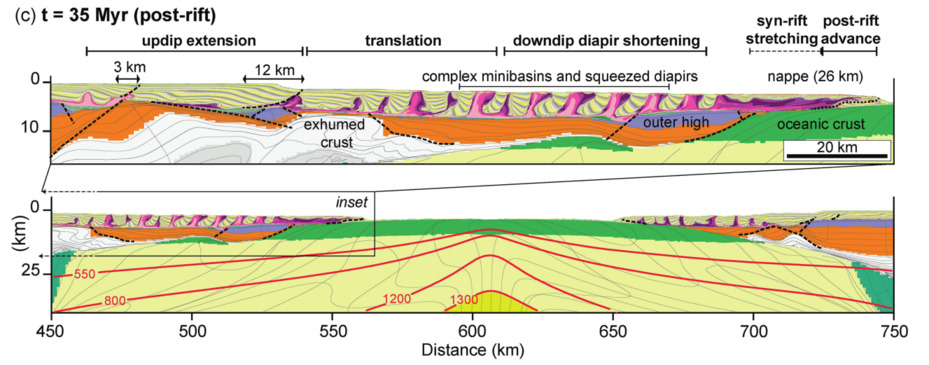
\includegraphics[height=5cm]{images/mycodes/pihg22a_img}
\end{center}

%--------------------------------------------------------------------------------------------------
\item {\it Coupling Crustal-Scale Rift Architecture With Passive Margin
Salt Tectonics: A Geodynamic Modeling Approach}, 
L.M. Pichel, R.S. Huismans, R. Gawthorpe, J.I. Faleide and Th. Theunissen, JGR, 127, 2022. \cite{pihg22b}
\begin{center}
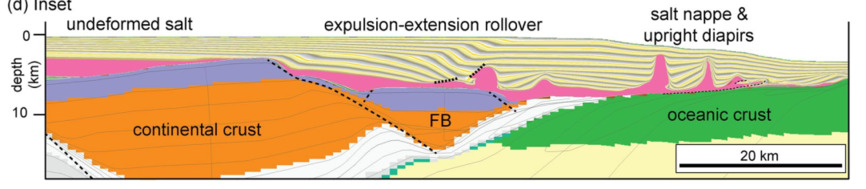
\includegraphics[height=3cm]{images/mycodes/pihg22b_img}
\end{center}

%--------------------------------------------------------------------------------------------------
\item {\it How post-­salt sediment flux and progradation rate
influence salt tectonics on rifted margins: Insights from
geodynamic modelling},
L.M. Pichel, R.S. Huismans, R. Gawthorpe and  J.I. Faleide, Basin Research, 2023. \cite{pihg23}
\begin{center}
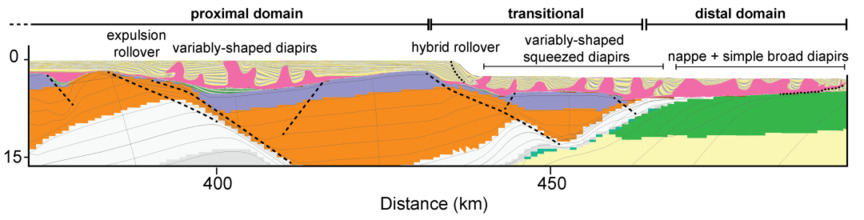
\includegraphics[height=3cm]{images/mycodes/pihg23_img}
\end{center}

\item {\it A Three-Field Formulation for Two-Phase Flow in
Geodynamic Modeling: Toward the Zero-Porosity Limit},
Gang Lu, Dave A. May and Ritske S. Huismans, 
Journal of Geophysical Research: Solid Earth, 2024. \cite{lumh24}


\end{itemize}


%--------------------------------------------------------------------------------------------------
%--------------------------------------------------------------------------------------------------
%--------------------------------------------------------------------------------------------------
%--------------------------------------------------------------------------------------------------

Upon my arrival at Utrecht University in 2012 I started working an a more flexible code, called \elefant, 
which has since very much diverged from \fantom.

\begin{itemize}
\item {\it The effect of obliquity on temperature in subduction zones: insights from 3-D numerical modeling}, 
A. Plunder, C. Thieulot and D.J.J. van Hinsbergen, Solid Earth 9, 759-776, 2018. \url{https://doi.org/10.5194/se-9-759-2018}

\begin{center}
\includegraphics[height=3.5cm]{images/mycodes/pltv18_img}
\end{center}


\item {\it Analytical solution for viscous incompressible Stokes flow in a spherical shell}, 
C. Thieulot, Solid Earth 8, 1181-1191, 2017. \url{https://doi.org/10.5194/se-8-1181-2017}

\begin{center}
\includegraphics[height=3cm]{images/mycodes/thie17_img}
\end{center}



\item  {\it Lithosphere erosion and continental breakup: interaction of extension, plume upwelling and melting}, 
A. Lavecchia, C. Thieulot, F. Beekman, S. Cloetingh and S. Clark, E.P.S.L. 467, p89-98, 2017.

\begin{center}
\includegraphics[height=3cm]{images/mycodes/latv17_img}
\end{center}


\item {\it Benchmarking numerical models of brittle thrust wedges}, 
Susanne J.H. Buiter, Guido Schreurs, Markus Albertz, Taras V. Gerya, Boris Kaus,
Walter Landry, Laetitia le Pourhiet, Yury Mishin, David L. Egholm, Michele Cooke,
Bertrand Maillot, Cedric Thieulot, Tony Crook, Dave May, Pauline Souloumiac, Christopher Beaumont
Journal of Structural Geology 92, p140-177, 2016. \url{https://doi:10.1016/j.jsg.2016.03.003}

\begin{center}
\includegraphics[height=1.8cm]{images/mycodes/busa16_img}
\end{center}


\item {\it A community benchmark for viscoplastic thermal convection in a 2-D square box}, 
N. Tosi, C. Stein, L. Noack, C. Huettig, P. Maierova, H. Samuel, D.R. Davies, C.R. Wilson, S.C. Kramer, C. Thieulot, A. Glerum, M. Fraters, W. Spakman, A. Rozel, P.J. Tackley, Geochem. Geophys. Geosyst. 16, doi:10.1002/2015GC005807, 2015.

\begin{center}
\includegraphics[height=3cm]{images/mycodes/tosn15_img}
\end{center}


\item {\it Dynamics of intraoceanic subduction initiation: 1. Oceanic detachment fault inversion and the formation of supra-subduction zone ophiolites}, M. Maffione, C. Thieulot, D.J.J. van Hinsbergen, A. Morris, O. Pluemper and W. Spakman, Geochem. Geophys. Geosyst. 16, p1753-1770, 2015.

\begin{center}
\includegraphics[height=1.8cm]{images/mycodes/matv15_img}
\end{center}

\item {\it The Geodynamic World Builder: a solution for complex initial conditions in numerical modelling},
M. Fraters, C. Thieulot, A. van den Berg and W. Spakman,
Solid Earth, \url{https://doi.org/10.5194/se-2019-24}, 2019.

\begin{center}
\includegraphics[height=2.8cm]{images/mycodes/frtv19_img}
\end{center}


\end{itemize}


\begin{itemize}
\item {\it GHOST: Geoscientific Hollow Sphere Tessellation}, 
C. Thieulot, Solid Earth, 9, 1169-1177, 2018. \url{https://doi.org/10.5194/se-9-1169-2018}

\begin{center}
\includegraphics[height=3cm]{images/mycodes/shell_HS06}
\includegraphics[height=3cm]{images/mycodes/shell_HS12}
\includegraphics[height=3cm]{images/mycodes/shell_HS20}
\end{center}


title={Long-term coupling and feedback between tectonics and surface processes 
during non-volcanic rifted margin formation},
author={Theunissen, Thomas and Huismans, Ritske S},
journal={Journal of Geophysical Research: Solid Earth},

\end{itemize}

